\documentclass[mat1]{fmfdelo}
% \documentclass[fin1]{fmfdelo}
% \documentclass[isrm1]{fmfdelo}
% \documentclass[mat2]{fmfdelo}
% \documentclass[fin2]{fmfdelo}
% \documentclass[isrm2]{fmfdelo}

\usepackage{graphicx}
\allowdisplaybreaks



% naslednje ukaze ustrezno napolnite
\avtor{Maruša Oražem}

\naslov{Konstrukcija gibanja kamere s pomočjo Pitagorejskih krivulj}
\title{Construction of camera motion with help of Pitagorean curves}

% navedite ime mentorja s polnim nazivom: doc.~dr.~Ime Priimek,
% izr.~prof.~dr.~Ime Priimek, prof.~dr.~Ime Priimek
% uporabite le tisti ukaz/ukaze, ki je/so za vas ustrezni
\mentor{izr. prof. dr. Marjetka Knez}
% \mentorica{}
% \somentor{}
% \somentorica{}
% \mentorja{}{}
% \mentorici{}{}

\letnica{2020} % leto diplome

%  V povzetku na kratko opišite vsebinske rezultate dela. Sem ne sodi razlaga organizacije dela --
%  v katerem poglavju/razdelku je kaj, pač pa le opis vsebine.
\povzetek{}

%  Prevod slovenskega povzetka v angleščino.
\abstract{}

% navedite vsaj eno klasifikacijsko oznako --
% dostopne so na www.ams.org/mathscinet/msc/msc2010.html
\klasifikacija{}
\kljucnebesede{} % navedite nekaj ključnih pojmov, ki nastopajo v delu
\keywords{} % angleški prevod ključnih besed

\zapisiMetaPodatke  % poskrbi za metapodatke in veljaven PDF/A-1b standard

% aktivirajte pakete, ki jih potrebujete
% \usepackage{tikz}

% za številske množice uporabite naslednje simbole
\newcommand{\R}{\mathbb R}
\newcommand{\N}{\mathbb N}
\newcommand{\Z}{\mathbb Z}
\newcommand{\C}{\mathbb C}
\newcommand{\Q}{\mathbb Q}
\newcommand{\HH}{\mathbb H}
\newcommand{\rr}{\boldsymbol r}
\newcommand{\ii}{\boldsymbol i}
\newcommand{\jj}{\boldsymbol j}
\newcommand{\kk}{\boldsymbol k}
\newcommand{\pp}{\boldsymbol p}
\newcommand{\ba}{\boldsymbol a}
\newcommand{\bb}{\boldsymbol b}
\newcommand{\e}{\boldsymbol e}
\newcommand{\oo}{\boldsymbol o}
\newcommand{\uu}{\boldsymbol u}
\newcommand{\vv}{\boldsymbol v}
\newcommand{\A}{\mathcal A}
\newcommand{\B}{\mathcal B}
\newcommand{\CC}{\mathcal C}
\newcommand{\QQ}{\mathcal Q}
\newcommand{\ff}{\boldsymbol f}
\newcommand{\g}{\boldsymbol g}
\newcommand{\TT}{\boldsymbol t}
\newcommand{\NN}{\boldsymbol n}
\newcommand{\BB}{\boldsymbol b}

% matematične operatorje deklarirajte kot take, da jih bo Latex pravilno stavil
% \DeclareMathOperator{\conv}{conv}

% vstavite svoje definicije ...
%  \newcommand{}{}

\begin{document}

\section{Uvod}
V današnjem času je kamera povsem vsakdanji predmet, ki ga srečamo na vsakem koraku. Vgrajena je v skoraj vsak prenosni telefon in računalnik. Dan danes lahko vsak posname nek objekt. Kako pa le tega posneti, da bo naš posnetek čim boljši? Tisti, ki se z posnetki ukvarjajo bolj profesonalno imajo na voljo pripomočke s pomočjo katerih lahko prehodijo neko pot in ob tej poti snemajo nek fiksen objekt. Poti po katerih lahko potuje kamera je seveda neskončno mnogo. Katera pa je najboljša, pa je odvisno od samega vprašanja.  Smiselno se je uprašati, kakšna naj bo predpisana pot kamere, da bo le ta vedno obrnjena proti objektu ki ga snemamo, da se kamera ne bo vrtela okoli svoje osi in s tem poskrbela da se slika ne bo po nepotrebnem vrtela. S takšnimi in podobnimi vprašanji se ukvarjajo predvsem ljudje, ki se ukvarjajo s snemanjem filmov, prav tako pa tudi v navideznem svetu oziroma v svetu računalniških igric. Aplikacije danega problema se uporabljajo celo v medicini in sicer pri endoskopskih operacijah, kjer kirurg vodi kamero do končnega objekta znotraj naših teles. Naš cilj bo opisati take poti kamere, kjer bo kamera ves čas obrnjena proti nekemu fiksnemu objektu in ga pri tem čimbolje posnela. Predpisali bomo začetek in konec krivulje, ki bo določala pot. Med vsemi možnimi krivuljami, bomo poiskali takšne, za katere obstaja taka orientacija, da bo naša kamera potovala brez nepotrebnih rotacij okoli osi, ki bo kazala proti objektu, ki ga snemamo.

V prvem delu diplome se bomo seznanili z osnovnimi pojmi in definicijami, ki jih bomo potrebovali. Nato bomo prepisali predpis, s katerim bomo dobili našo krivuljo in si ogledali kako izbira točk vpliva na sam izgled krivulje. Ogledali si bomo razliko med usmerjenimi in prikrojenimi ogrodji, ter ogrodji ki minimizirajo vrtenje okoli prve osi v ogrodju. Na koncu pa bomo naše ugotovitve ponazorili z primeri.

%%%%%%%%%%%%%%%%%%%%%%%%%%%%%%%%%%%%%%%%%%%%%%%%%%%%%%%%%%%%%%%%%%%%%%%%%%%%%%%%%%%%%%%%%%%%%%%%%%%%%%%%
\section{Osnovni pojmi in definicije}
Za začetek se spoznajmo z osnovnimi pojmi in definicijami, ki jih bomo potrebovali v nadaljevanju.
\begin{definicija}
Množica kvaternionov $\HH$ je 4-razsežen vektorski prostor z bazo $\bf{1},\bf{i},\bf{j},\bf{k}$.
\end{definicija}
Vsak kvaternion $\A \in \HH$ lahko zapišemo kot $\A = a_0 + a_1\mathbf{i} + a_2\mathbf{j} + a_3\mathbf{k}$ oziroma $\A=(a_0,a_1,a_2,a_3)$, kjer so $a_0,a_1,a_2,a_3\in \R$ ali pa kot skalarni in vektorski del $\A =(a_0,\boldsymbol{a})$, kjer je $\A = (a_1,a_2,a_3)$.
Poglejmo si osnovne operacije v množici $\HH$:\\
\begin{itemize}
\item Seštevanje:
\begin{equation*}
\begin{split}
\A + \B &= (a_0+b_0,a_1+b_1,a_2+b_2,a_3+b_3)  \\
 		  &=(a_0+b_0) + (a_1+b_1)\mathbf{i} + (a_2+b_2)\mathbf{j} + (a_3+b_3)\mathbf{k}, \\
 		  &  		  \A = (a_0,a_1,a_2,a_3) \in \HH, \quad \B = (b_0,b_1,b_2,b_3) \in \HH.
\end{split}
\end{equation*}
\item Skalarno množenje:
\begin{equation*}
\lambda \A = (\lambda a_0, \lambda a_1, \lambda a_2, \lambda a_3) =  \lambda a_0 + \lambda a_1 \mathbf{i} + \lambda a_2 \mathbf{j} + \lambda a_3 \mathbf{k}, \quad \lambda \in \R,\quad \A \in \HH.
\end{equation*}
\item Konjugacija:
\begin{equation*}
\overline{\A} = (a_0,-a_1,-a_2,-a_3)= a_0-a_1\mathbf{i} - a_2\mathbf{j} - a_3\mathbf{k}, \quad \A \in \HH .
\end{equation*}
\item Kvaternionsko množenje:
$\text{Velja zveza:}~\mathbf{i}^2 = \mathbf{j}^2 = \mathbf{k}^2 = \mathbf{ijk} = -1$. Iz te zveze sledijo formule za posamezno množenje dveh baznih elementov. Od koder izpeljemo
\begin{equation*}
\begin{split}
\A \cdot \B &= (a_0 + a_1\ii +a_2\jj+a_3\kk)(b_0+b_1\ii+b_2\jj+b_3\kk) \\
&=a_0b_0+a_0b_1\ii+a_0b_2\jj+a_0b_3\kk+a_1b_0\ii+a_1b_1\ii^2+a_1b_2\ii\jj+a_1b_3\ii\kk+a_2b_0\jj\\
&+a_2b_1\jj\ii+a_2b_2\jj^2+a_2b_3\jj\kk+a_3b_0\kk+a_3b_1\kk\ii+a_3b_2\kk\jj+a_3b_3\kk^2\\
&=(a_0b_0-a_1b_1-a_2b_2-a_3b_3) +(a_0b_1+a_1b_0+a_2b_3-a_3b_2)\ii \\
&+(a_0b_2-a_1b_3+a_2b_0+a_3b_1)\jj +(a_0b_3+a_1b_2-a_2b_1+a_3b_0)\kk,\\
&\A = (a_0,a_1,a_2,a_3) \in \HH, \quad \B = (b_0,b_1,b_2,b_3) \in \HH.
\end{split}
\end{equation*}
Če kvaternione pišemo v obliki $\A=(a,\ba)$ in $\B=(b,\bb)$, se formula za množenje zapiše krajše kot
\begin{equation}{\label{mn_kvat}}
	\A \cdot \B = \left( ab-\langle \ba,\bb \rangle, a\bb-b\ba-\ba \times \bb\right)
\end{equation}
\end{itemize}
Zaradi lažjega razumevanja, bomo kvaternionsko množenje označevali z $\cdot$, skalarno množenje pa z $\langle\cdot,\cdot\rangle$.
\begin{primer}
	Primer uporabe formule za kvaternionsko množenje . Izpeljali bomo formulo za  množenje dveh kvaternionov, ki imata skalarni del enak 0.
	Naj bosta $\A = (0,\boldsymbol{a})$ in $\B=(0,\boldsymbol{b})$. Po formuli \ref{mn_kvat} dobimo
	\begin{equation*}
	(0,\boldsymbol{a}) \cdot (0,\boldsymbol{b}) = \left( -\langle \boldsymbol{a}, \boldsymbol{b} \rangle , -\boldsymbol{a} \times \boldsymbol{b} \right),
	\end{equation*}
	od koder sledi,da je
	\begin{equation}{\label{mn_kvat_0}}
	\langle \boldsymbol{a},\boldsymbol{b} \rangle = -{\rm scal}\left( (0,\boldsymbol{a}) \cdot (0,\boldsymbol{b}) \right).
	\end{equation}
\end{primer}
\begin{opomba}
	Oznaka ${\rm scal}(\cdot)$ označuje skalarni del produkta. Z ${\rm vect}(\cdot)$ pa bomo označili vektorski del. Torej če je $\A = (a,\ba)$, označimo ${\rm scal}(\A) = a$ in ${\rm vect}(\A)=\ba$.
\end{opomba}
\begin{opomba}
	Kvaternionu, ki ima skalarni del enak 0, rečemo čisti kvaternion.
\end{opomba}
Normo kvaterniona $\A$ izračunamo kot
\begin{equation*}
||\A|| = \sqrt{\langle \A, \overline{\A}\rangle}, \quad \A \in \HH.
\end{equation*}
\begin{definicija}
\textit{Parametrično podana krivulja} v $\R^d$ je množica točk, podana s parametrizacijo
\begin{equation*}
\rr: [ a,b ] \rightarrow \R^d, \quad t ~ \longmapsto ~\rr(t) = \left( r_1(t),r_2(t), \dots, r_d(t)\right)
\end{equation*}
\end{definicija}
\begin{definicija}
	Krivulja $\rr$ je \textit{racionalna}, če velja $\rr(t) = \frac{\pp(t)}{\boldsymbol{q}(t)}$, kjer sta $\pp$ in $\boldsymbol{q}$ polinoma.
\end{definicija}
V nadaljevanju se bomo omejili na prostorske krivulje. V tem primeru bodo parametrizacije oblike $\rr(t) = \left( x(t),y(t),z(t) \right)$.
\begin{definicija}
Parametrično podana krivulja $\rr$ je \textit{Pitagorejska krivulja\\ (P-krivulja)}, če je $\boldsymbol{o}(t) = \frac{\rr(t)}{||\rr(t)||}$ racionalna, oziroma če je $||\rr(t)|| = \sigma(t)$ za nek polinom $\sigma$ .
\end{definicija}
\begin{definicija}
	Z $\mathbb{P}_n$ označimo prostor polinomov stopnje največ $n$.
\end{definicija}


%%%%%%%%%%%%%%%%%%%%%%%%%%%%%%%%%%%%%%%%%%%%%%%%%%%%%%%%%%%%%%%%%%%%%%%%%%%%%%%%%%%%%%%%%%%%%%%%%%%%%%%%%%%
\section{Konstrukcija P-krivulje}
V tem razdelku bomo opisali postopek, s katerim bomo dobili krivuljo.\\
Za začetek vzemimo poljubnen kvaternionski polinom $\mathcal{A}(t)$, ki naj bo stopnje $n$. Torej
\begin{equation*}
\mathcal{A}: I \subset \R \rightarrow \HH,
\end{equation*}
\begin{equation*}
\mathcal{A}(t) = u(t) + v(t) \mathbf{i} + p(t) \mathbf{j} + q(t) \mathbf{k}, \quad t \in I,\quad u,v,p,q \in \mathbb{P}_n.
\end{equation*}
Iz kvaternionskega polinoma $\mathcal{A}(t)$ bomo konstruirali parametrično krivuljo $\mathbf{p}(t)$ in sicer naj bo
\begin{equation}
\boldsymbol{p}(t) = \mathcal{A}(t) \boldsymbol{i} \overline{\mathcal{A}}(t).
\end{equation}
Pokažimo, da je tako dobljena krivulja res parametrična polinomska P-krivulja. Izkaže se, da je stopnje $2n$. Zaradi boljše preglednosti bomo izpustili argument, vendar se zavedamo, da so predpisi odvisni od parametra t.Dobimo
\begin{equation*}
\begin{split}
\mathcal{A}\boldsymbol{i}\overline{\mathcal{A}} & =(u\boldsymbol{i}-v-p\boldsymbol{k}+q\boldsymbol{j})(u-v\boldsymbol{i}-p\boldsymbol{j}-q\boldsymbol{k}) \\
&= u^2 \ii -uv\ii^2-pu\ii\jj - uq\ii\kk - vu + v^2\ii + vp\jj\\
&~~ +vq\kk - pu\kk + pv\kk\ii + p^2 \kk\jj + pq\kk^2 + qu\jj - qv\jj\ii - qp\jj^2 -q^2\jj\kk \\
& = u^2\ii + uv - pu\kk + uq\jj -vu+v^2\ii +vp\jj + vq\kk \\
& ~~-pu\kk+pv\jj-p^2\ii-pq+qu\jj+qv\kk+qp-q^2\ii \\
& = (u^2+v^2-p^2-q^2)\ii + 2(uq-vp)\jj +2(vq-pu)\kk.
\end{split}
\end{equation*}
Opazimo, da je skalarni del enak 0, zato lahko $\pp = \A\ii\A$ identificiramo s krivuljo v $\R^3$. Torej dobimo
\begin{equation*}
\pp = (u^2+v^2-p^2-q^2, 2(uq+vp),2(vq-pu)).
\end{equation*}
Ker smo predpostavili, da so v kvaternionskemu polinomu $\A=u+v\ii+p\jj+q\kk$ funkcije $u,v,p,q$ polinomi stopnje $n$, in ker v $\pp$ nastopajo le zmnožki dveh od teh polinomov, vsote in razlike, je dobljena krivulja $\pp$ polinom stopnje $2n$.\\
Pokažimo sedaj, da je krivulja $\pp$, dobljena po zgornjem predpisu res P-krivulja. Dokazati moramo, da je $\boldsymbol{o} = \frac{\pp}{||\pp||}$ racionalna krivulja. Vemo že, da je $\pp$ polinom. Preverimo, da je tudi $||\pp||$ polinom. Dobimo
\begin{equation*}
\begin{split}
||\pp||^2 &= \langle \pp,\overline{\pp}\rangle = (\A\ii\overline{\A})\overline{(\A\ii\overline{\A})} \\
&= \A\ii\overline{\A}\A\overline{\ii} \overline{\A} \\
&= ||\A||^2 \A \ii \overline{\ii} \overline{\A} \\
& = ||\A||^2 \A \overline{\A} \\
&=||\A||^4.
\end{split}
\end{equation*}
Torej je $||\pp|| = ||\A||^2$. Ker je $\A$ sestavljen iz polinomov, je $||\pp||$ res polinom.\\

\begin{lema}
	Iz kvaternionskega polinoma $\A(t)$, stopnje $n$, smo po predpisu\\ $\pp(t) = \A(t)\ii\overline{\A(t)}$ konstruirali P-krivuljo stopnje $2n$. 
\end{lema}

\subsection{Zapis krivulje v Bernsteinovi bazi}
Naš cilj je opisati gibanje kamere okoli nekega fiksnega objekta. Gibanje kamere bo določeno s prostorsko krivuljo, opremljeno z ortonormiranim ogrodjem. Ker želimo, da bo gibanje opisano z racionalnimi funkcijami, moramo za krivuljo izbrati polinomsko/racionalno krivuljo, ki se jo da opremiti z racionalnim ortonormiranim ogrodjem. Želimo si nadzorovati to gibanje in vsaj pribljižno napovedati, kje se bo krivulja gibala. Videli bomo, da tega ne moremo doseči, če polinomsko krivuljo zapišemo v standardni bazi. To bomo dosegli s pomočjo Bernsteinove baze vektorskega prostora $\mathbb{P}_n$. \\
Poglejmo si najprej zapis krivulje v standardni bazi. Poljuben polinom $\pp$ stopnje $n$, se v standardni bazi zapiše kot
\begin{equation*}
\pp(t) = \sum_{i=0}^n \pp_i t^i \quad \text{kjer so $p_i$ točke v $\R^3$.}
\end{equation*}
Poglejmo si nekaj preprostih primerov, kjer primerjamo izbrane točke $\pp_i$ in obliko dobljene krivulje $\pp(t)$.

\begin{figure}[ht!]

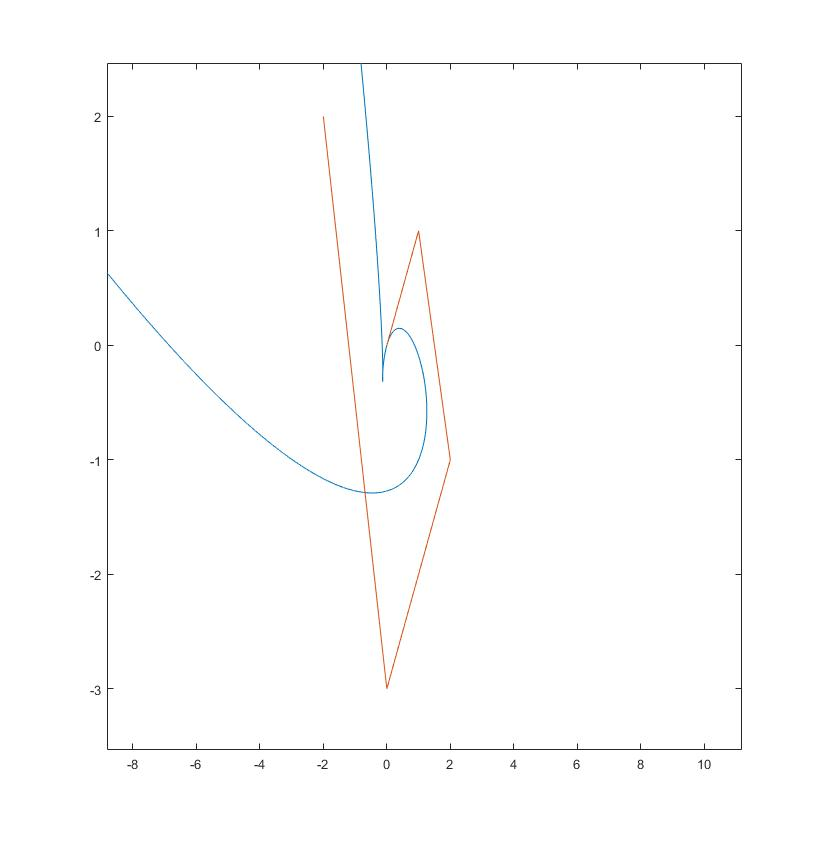
\includegraphics[scale=0.20]{C:/Users/Acer/Desktop/diploma/Diploma/slike/standKrivulja3.jpg}{a}

\end{figure}
 \begin{figure}[ht!]
 	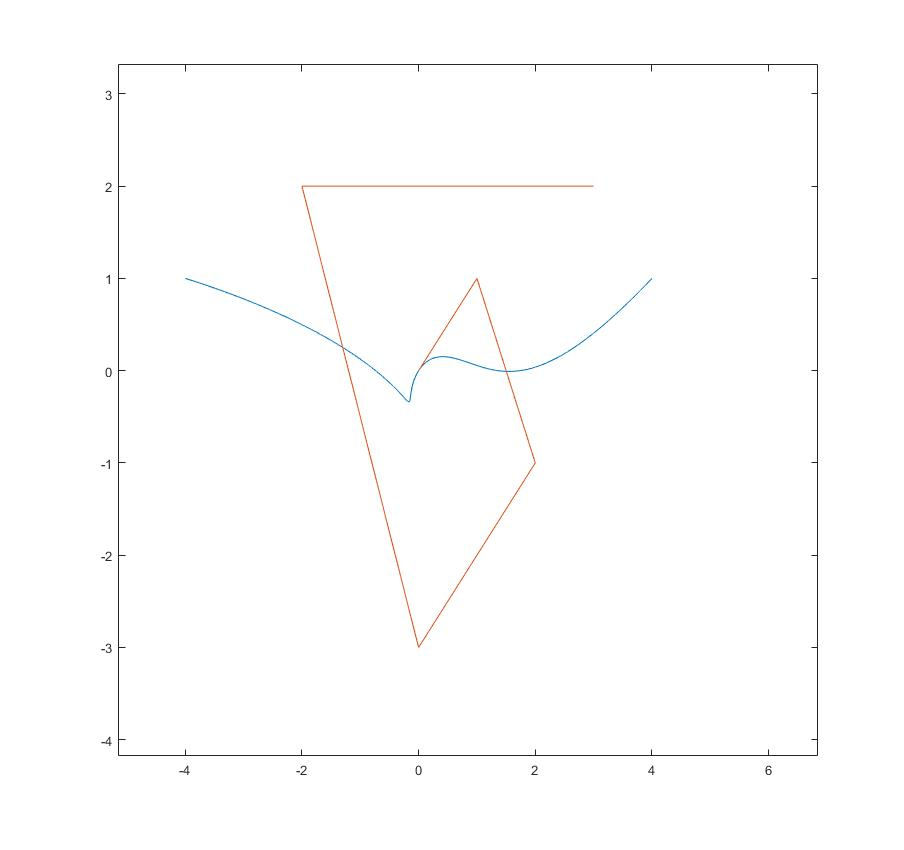
\includegraphics[scale=0.20]{C:/Users/Acer/Desktop/diploma/Diploma/slike/standKrivulja4.jpg}
 	\caption{desna slika}
 \end{figure}


Na slikah \ref{stand_1} in \ref{stand_2} so z oranžno barvo narisane in povezane izbrane točke $p_i$, z modro pa je prikazana dobljena krivulja $\pp(t)$, zapisana v standardni bazi.
Vidimo, da med izbranimi točkami in obliko krivulje ni vidne povezave. \\

Poglejmo si, kako je definirana Bernsteinova baza in kakšno povezavo imajo točke z obliko krivulje.
\begin{definicija}
Bernsteinovi bazni polinomi, stopnje $n$, so
\begin{equation*}
B_i^n(t) = \binom{n}{i} t^i (1-t)^{n-i}, \quad i=0,1,\dots,n,
\end{equation*}
kjer je $t\in\left[0,1\right]$.
\end{definicija}
\begin{equation*}
\begin{array}{c c}
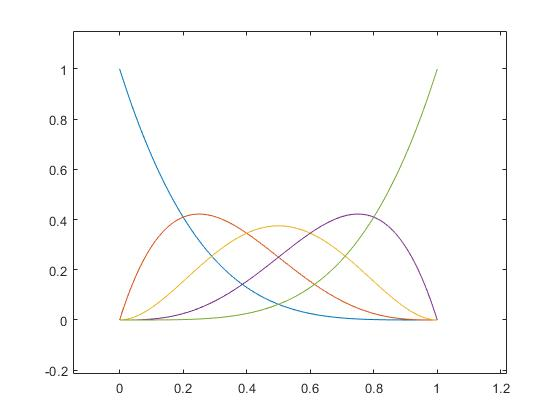
\includegraphics[scale=0.35]{C:/Users/Acer/Desktop/diploma/Diploma/slike/bernPolinom4.jpg} &
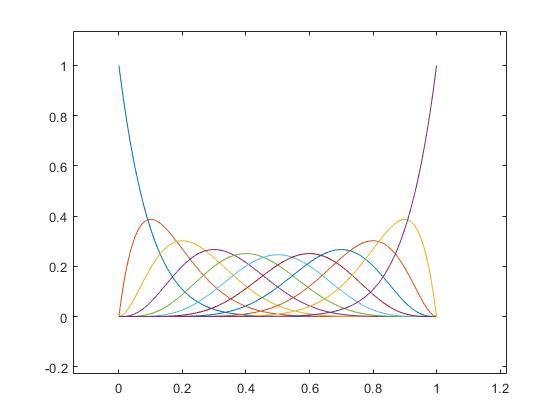
\includegraphics[scale=0.35]{C:/Users/Acer/Desktop/diploma/Diploma/slike/bernPolinom10.jpg}
\end{array}
\end{equation*}
Sliki \ref{bern_1} in \ref{bern_2} prikazujeta Bernsteinove bazne polinome za $n = 4$ in $n= 10$.
\begin{trditev}
	Bernsteinovi bazni polinomi stopnje $n$, tvorijo bazo za $\mathbb{P}_n$.
\end{trditev}
Predno se lotimo dokaza, zapišimo še lemi, ki ju bomo potrebovali v dokazu.
\begin{lema}
	Velja naslednja enakost:
	\begin{equation}{\label{binom}}
		\binom{n}{i} \binom{n-i}{j-i} = \binom{n}{j} \binom{j}{i}.
	\end{equation}
\end{lema}
\begin{dokaz}
	Razpišemo vsako stran posebej in ju primerjamo. Leva stran nam da
	\begin{equation*}
		\frac{n!}{i!(n-i)!} \frac{(n-i)!}{(j-i)!(n-i-j+i)!} = \frac{n!}{i!(j-i)!(n-j)!}.
	\end{equation*}
	Desna stran nam da
	\begin{equation*}
		\frac{n!}{j!(n-j)!} \frac{j!}{i!(j-i!)} = \frac{n!}{(n-j)!i!(j-i)!}.
	\end{equation*}
	Vidimo, da enačba drži.
\end{dokaz}
\begin{lema}{\label{bern_potencna}}
	Bernsteinovi bazni polinomi $B_i^n$ se v potenčni bazi izražajo kot
	\begin{equation}{\label{bern_pot}}
		B_i^n(t) = \sum_{j=i}^n (-1)^{j-i} \binom{n}{j} \binom{j}{i} t^j.
	\end{equation}
\end{lema}
\begin{dokaz}
	Za dokaz uporabimo binomski izrek, ki pove razvoj potence binoma in sicer
	\begin{equation*}
		\left(x + y\right)^n = \sum_{i=0}^n \binom{n}{i}x^{n-i}y^i.
	\end{equation*}
	Zapišimo Bernsteinov bazni polinom po definiciji in upoštevajmo razvoj potence binoma. Torej
	\begin{equation*}
	\begin{split}
	B_i^n(t) &= \binom{n}{i}t^i\left(1-t\right)^{n-i} = \binom{n}{i}t^i \sum_{j=0}^{n-i} \binom{n-i}{j}1^{n-i-j}(-t)^j \\
	&= \sum_{j=0}^{n-i} \binom{n}{i} \binom{n-i}{j} (-1)^j t^{i+j}.
	\end{split}
	\end{equation*}
	Zamaknemo indeks v vsoti in dobimo
	\begin{equation*}
		B_i^n(t) = \sum_{j=i}^{n} \binom{n}{i} \binom{n-i}{j-i} (-1)^{j-i} t^{j}.
	\end{equation*}
	Upoštevamo enačbo \ref{binom} in dobimo
	\begin{equation*}
		B_i^n(t) = \sum_{j=i}^n \binom{n}{j} \binom{j}{i} (-1)^{j-i} t^j,
	\end{equation*}
	kar zaključuje dokaz.
\end{dokaz}
\begin{dokaz}
	Ker je število Bernsteinovih baznih polinomov enako dimenziji prostora $\mathbb{P}_n$, je potreba dokazati le, da so med sabo linearno neodvisni. Torej pokazati moramo, da je
	\begin{equation*}
		\sum_{i=0}^n \alpha_i B_i^n = 0 \quad \Longleftrightarrow \quad \alpha_i = 0, \quad \forall i.
	\end{equation*}
	Linearno neodvisnost bomo pokazali tako, da bomo zapisali preslikavo, ki bo preslikala standardno bazo za $\mathbb{P}_n$ v Bernsteinovo bazo. Ker vemo da je standardna baza linearno neodvisna, bo sledilo da so neodvisni tudi Bernsteinovi bazni polinomi. Uporabimo lemo \ref{bern_potencna} in zapišemo
	\begin{equation*}
		\begin{bmatrix}
		B_0^n(t) \\ \\B_1^n(t) \\ \\ \vdots \\ \\ B_n^n(t)
		\end{bmatrix}
		= 
		\begin{bmatrix}
		\binom{n}{0} & -\binom{n}{1} & \binom{n}{2} &\cdots &(-1)^n \binom{n}{n} \\ \\
		0 & \binom{n}{1} \binom{1}{1} &-\binom{n}{2} \binom{2}{1} &\cdots & (-1)^{n-1} \binom{n}{n} \binom{n}{1} \\ \\
		\vdots &&&\ddots& \vdots \\ \\
		0 &0& 0 & \cdots & 1
		\end{bmatrix}
		\begin{bmatrix}
		1 \\ \\ t  \\ \\ \vdots \\ \\ t^n
		\end{bmatrix}.
	\end{equation*}
	Pokazati moramo, da je prehodna matrika obrljiva. Označimo jo z $A$. Ker je $A$ zgornjetrikotna, moramo pokazati le, da so diagonalni elementi neničelni, kar pa očitno drži. Torej obstaja inverzna matrika $A^{-1}$, za katero velja
	\begin{equation*}
		\begin{bmatrix}
		1 \\   \\  t \\ \\ \vdots \\ \\ t^n
		\end{bmatrix}
		= A^{-1}
		\begin{bmatrix}
		B_0^n(t) \\ \\B_1^n(t) \\ \\ \vdots \\ \\ B_n^n(t)
		\end{bmatrix}.		
	\end{equation*}
	Torej so Bernstenovi bazni polinomi res linearno neodvisni in tvorijo bazo za $\mathbb{P}_n$.
\end{dokaz}
Poglejmo si nekaj lastnosti Bernsteinovih polinomov.
\begin{itemize}
	\item Bernsteinovi bazni polinomi so nenegativni na intervalu $\left[0,1\right]$.
	\item Velja:
	\begin{equation*}
		\sum_{i=0}^n B_i^n(t) = 1, \quad t\in \R.
	\end{equation*}
	\item Bernsteinovi bazni polinomi so simetrični. Torej velja
	\begin{equation*}
		B_i^n(t) = B_{n-i}^n(1-t), \quad t\in\R.
	\end{equation*}
	\item Prva in zadnja točka določata začetek in konec krivulje, medtem ko umesne točke določajo obliko krivulje.
\end{itemize}
Ker si želimo nadzorovati obliko krivulje, bo za nas najpomembnejša zadnja lastnost. Le to prikazujeta sliki \ref{label} in \ref{label}.
Zapišimo sedaj poljubno krivuljo $\pp(t)$ v Bernsteinovi bazi. Dobimo
\begin{equation*}
\pp(t) = \sum_{i=0}^n \pp_i B_i^n(t),
\end{equation*}
kjer so $\pp_i \in \R^3$ in $B_i^n$ Bernsteinovi bazni polinomi. Točkam $\pp_i$ rečemo kontrolne točke, te pa tvorijo tako imenovani kontrolni poligon, ki določa obliko krivulje.

\begin{equation*}
\begin{array}{c c}
\includegraphics[scale=0.35]{C:/Users/Acer/Desktop/diploma/Diploma/slike/bernKrivulja1.jpg} &
\includegraphics[scale=0.15]{C:/Users/Acer/Desktop/diploma/Diploma/slike/bernKrivulja3.jpg}
\end{array}
\end{equation*}
Sliki \ref{bbaza_1} in \ref{bbaza_2} nam prikazujeta krivuljo, dobljeno iz kontrolnih točk in zapisano v Bernsteinovi bazi. Vidimo, da če si narišemo kontrolni poligon (oranžna barva), se krivulja (modra barva) začne v prvi kontrolni točki in konča v zadnji. Pot krivulje med tema dvema točkama, pa poteka po notranjosti mnogokotnika, ki ga določa kontrolni poligon.
\iffalse
Primer prileganja krivulje kontrolnemu poligoni na točkah (0,0), (1,1), (2,-1), (0,-3), (-2,2) in če dodamo še (3,2).
\fi
\begin{primer}Za $n = 2$ dobimo
\begin{equation*}
B_i^2(t) = \binom{2}{i} t^i(1-t)^{2-i}, \quad i=0,1,2.
\end{equation*}
Če razpišemo za vsak $i$ dobimo
\begin{equation*}
\begin{split}
B_0^2(t) &= \binom{2}{0} t^0(1-t)^{2-0} = (1-t)^2,\\
B_1^2(t) &= \binom{2}{1} t^1(1-t)^{2-1} = 2t(1-t),\\
B_2^2(t) &= \binom{2}{2} t^2(1-t)^{2-2} = t^2.
\end{split}
\end{equation*}
Torej lahko krivuljo $\pp$, stopnje 2, zapišemo kot
\begin{equation*}
	\pp(t) = \pp_0(1-t)^2 + \pp_1 2t(1-t) + \pp_2t^2,
\end{equation*}
kjer so $\pp_0, \pp_1, \pp_2 \in \R^3$. 
\begin{equation*}
\begin{array}{c c}
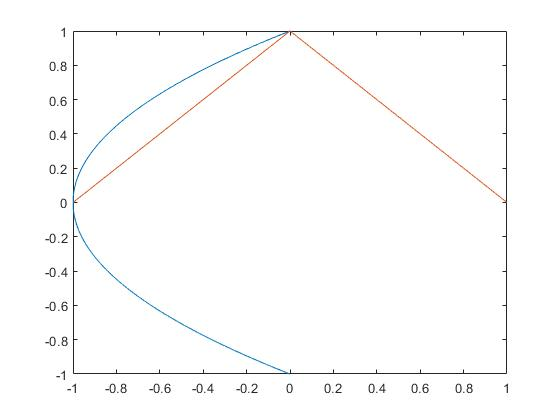
\includegraphics[scale=0.35]{C:/Users/Acer/Desktop/diploma/Diploma/slike/stand3.jpg} &
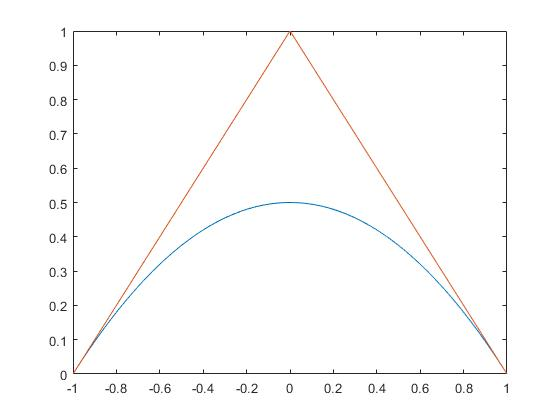
\includegraphics[scale=0.35]{C:/Users/Acer/Desktop/diploma/Diploma/slike/bern3.jpg}
\end{array}
\end{equation*}
Na zgornjih dveh slikah sta prikazani krivulji, ki jih dobimo, če vzamemo enake kontrolne točke in določimo krivuljo v standarni bazi (leva slika) in v Bernsteinovi bazi (desna slika). Kot smo že ugotovili zgoraj, je dobljena oblika lepša, če je krivulja zapisana v Bernsteinovi bazi. Nadzorujemo lahko začetno in končno točko, ter obliko krivulje.
\end{primer}



\subsection{Določitev kontrolnih točk P-krivulj}
V tem razdelku si bomo pogledali, kako določiti kontrolne točke za krivuljo, zapisano v Bernsteinovi bazi. P-krivuljo dobimo kot $\pp(t)=\A(t)\ii\overline{\A}$. V prejšnjem poglavju smo si pogledali kako zapišemo krivuljo v Bernsteinovi bazi. Tudi kvaternionski polinom $\A(t)$ bomo zapisali v Bernsteinovi bazi. Vprašanje je, kakšni naj bodo začetni koeficienti polinoma $\A(t)$, če določimo koeficiente krivulji $\pp(t)$. Torej, izbrane imamo točke, ki nam določajo obliko poti krivulje. Kakšni naj bodo potem koeficienti začetnega polinoma $\A(t)$? V nadaljevanju tega podpoglavja, bomo izpeljali kontrolne točke kriviljue $\pp$, ki jih dobimo iz kvaternionskih polinomov stopenj $1$, $2$ in $3$.
\begin{primer}{\label{primer35}}Poračunajmo Bernsteinove bazne polinome za $n=1$. Dobimo
\begin{equation*}
B_i^1(t) = \binom{1}{i} t^i(1-t)^{1-i}, \quad i= 0,1.
\end{equation*}
Iz česar sledi
\begin{equation*}
	\begin{split}
	B_0^1(t) &= \binom{1}{0} t^0(1-t)^{1-0} = 1-t, \\
	B_1^1(t) &= \binom{1}{1} t^1(1-t)^{1-1} = t.
	\end{split}
\end{equation*}
Torej se kvaternionski polinom $\A(t)$ prve stopnje zapiše kot
\begin{equation*}
\A(t) = \boldsymbol{A}_0(1-t) + \boldsymbol{A}_1t.
\end{equation*} 
Rekli smo, da je $\pp(t) = \A(t) \ii \overline{\A(t)}$. Vemo, da se splošni polinom stopnje n, v Bernsteinovi bazi, zapiše kot:
\begin{equation*}
\pp(t) = \sum_{k=0}^n \pp_k \binom{n}{k}(1-t)^{n-k}t^k.
\end{equation*}
Pokazali smo, da če je $\A$ stopnje $n$, bo $\pp = \A\ii\overline{\A}$ stopnje $2n$. Bernsteinovi bazni polinomi za $n=2$ so
\begin{equation*}
\begin{split}
B_0^2(t)& = (1-t)^2\\
B_1^2(t) &= 2t(1-t)\\
B_2^2(t) &= t^2.
\end{split}
\end{equation*}
Od tod sledi, da se $\pp(t)$ zapiše kot
\begin{equation*}
	\pp(t) = \sum_{i=0}^2 \pp_i B_i^2 = \pp_0 (1-t)^2 + \pp_12t(1-t) + \pp_2t^2,
\end{equation*}
kjer so $\pp_0,\pp_1,\pp_2 \in \HH$.
Razpišemo krivuljo $\pp(t)$ po definiciji in dobimo
\begin{equation*}
\begin{split}
\pp(t) &= \A(t)\ii\overline{\A(t)} \\
&= (\boldsymbol{A}_0(1-t) + \boldsymbol{A}_1t) \ii ( \overline{\boldsymbol{A}_0}(1-t) + \overline{\boldsymbol{A}_1}t) \\
& = (\boldsymbol{A}_0(1-t) + \boldsymbol{A}_1t) (\ii\overline{\boldsymbol{A}_0}(1-t) + \ii\overline{\boldsymbol{A}_1}t) \\
&=\A_0 \ii \overline{\A_0} (1-t)^2 + \A_0\ii\overline{\A_1}(1-t)t + \A_1\ii\overline{\A_0}t(1-t) + \A_1\ii\overline{\A_1}t^2 \\
&= \A_0 \ii \overline{\A_0} (1-t)^2 + \left(\frac{1}{2}\A_0\ii\overline{\A_1} +\frac{1}{2} \A_1\ii\overline{\A_0}\right)2t(1-t) + \A_1\ii\overline{\A_1}t^2.
\end{split}
\end{equation*}
Primerjamo istoležne koeficiente in dobimo naslednje enačbe:
\begin{equation*}
\begin{split}
\pp_0&= \A_0\ii\overline{\A_0}, \\
\pp_1&= \frac{1}{2}\left( \A_0\ii\A_1\overline{\A_1} + \A_1\ii\overline{\A_0}\right),\\
\pp_2&= \A_1\ii\overline{\A_1}.
\end{split}
\end{equation*}
\end{primer}
Z podobnim računanjem pridemo do kontrolnih točk P-krivulj višjih stopenj.
\begin{primer}Poglejmo si primer za $n=2$. Vemo, da bo krivulja $\pp$ stopnje 4.
Imamo kvaternionski polinom
\begin{equation*}
	\A(t) = \A_0(1-t)^2 + \A_12t(1-t) + \A_2(1-t)^2.
\end{equation*}
Želimo izračunati kontrolne točke za krivuljo
\begin{equation*}
	\pp(t) = \sum_{k=0}^4\pp_iB_i^4(t).
\end{equation*}
Kontrolne točke izračunamo po enakem postopku kot v primeru \ref{primer35} . Dobimo
\begin{equation*}
\begin{split}
\pp_0 & = \A_0\ii\overline{\A_0}, \\
\pp_1 &= \frac{1}{2}\left( \A_0\ii\overline{\A_1} + \A_1\ii\overline{\A_0} \right), \\
\pp_2 &= \frac{1}{6} \left( \A_0\ii\overline{\A_2} + 4\A_1\ii\overline{\A_1}+\A_2\ii\overline{\A_0} \right), \\
\pp_3 &= \frac{1}{2} \left( \A_1\ii\overline{\A_2}+\A_2\ii\overline{\A_1} \right), \\
\pp_4 &= \A_2\ii\overline{\A_2}.
\end{split}
\end{equation*}
\end{primer}

\begin{primer}
	Nazadnje si poglejmo še primer ko je $n=3$. Torej bomo dobili kontrole točke za krivuljo stopnje $6$. Kvaternionski polinom $\A$ je torej enak
	\begin{equation*}
	\A(t) = \A_0(1-t)^3+\A_13(1-t)^2t+\A_23(1-t)t^2+\A_3t^3.
	\end{equation*}
	Kot v primeru \ref{primer35} poračunamo in dobimo
	\begin{equation*}
	\begin{split}
	\pp_0 &= \A_0\ii\overline{\A_0} \\
	\pp_1 &= \frac{1}{2} (\A_0\ii\overline{\A_1}+\A_1\ii\overline{\A_0}) \\
	\pp_2 &= \frac{1}{5} (\A_0\ii\overline{\A_2} + 3\A_1\ii\overline{\A_1} + \A_2 \ii \overline{\A_0}) \\
	\pp_3 &= \frac{1}{20} (\A_0\ii\overline{\A_3}+9\A_1\ii\overline{\A_2}+9\A_2\ii\overline{\A_1}+\A_3\ii\overline{\A_0}) \\
	\pp_4&= \frac{1}{5} (\A_1\ii\overline{\A_3}+3\A_2\ii\overline{\A_2}+\A_3\ii\overline{\A_1}) \\
	\pp_5 &= \frac{1}{2} (\A_2\ii\overline{\A_3}+\A_3\ii\overline{\A_2}) \\
	\pp_6 &= \A_3 \ii \overline{\A_3}.
	\end{split}
	\end{equation*}
\end{primer}
Sedaj, ko imamo izračunane kontrolne točke, lahko iz njih izračunamo začetne koeficiente polinoma $\A$. Na primer, lahko si izberemo začetno in končno točko krivulje $\pp(0)$ in $\pp(1)$, od koder določimo kvaterniona $\A_0$ in  $\A_n$, kot je razloženo v nadaljevanju.
\begin{primer}Poglejmo si primer za	$n=1$. Nastavimo začetno in končno točko in dobimo
	\begin{equation}{\label{enacba}}
	\begin{split}
		\A_0\ii\overline{\A_0} &= \pp(0), \\
		\A_1\ii\overline{\A_1} &= \pp(1).
	\end{split}
\end{equation}
Iz teh dveh enačb lahko izrazimo $\A_0$ in $\A_1$ in dobimo začetni kvaternionski polinom $\A$. Podobno za polinome višjih stopenj, kjer si lahko izberemo začetno in končno točko ter še dodatno točko.	
\end{primer}
Poglejmo si kakšne so rešitve enačb oblike \ref{enacba}.
\begin{trditev}
	Naj bo $\A \in \HH$, $\CC$ čisti ne ničelni kvaternion. Rešitev enačbe 
	\begin{equation}{\label{aia}}
		\A \ii \overline{\A} = \CC
	\end{equation}
	 je
	\begin{equation}{\label{kvat_resitev}}
		\A(\phi) = \sqrt{||\CC||} \frac{\frac{\CC}{||\CC||} + \ii}{||\frac{\CC}{||\CC||} + \ii||} \mathcal{U}(\phi),
	\end{equation}
	kjer je $\mathcal{U}(\phi) = (\cos\phi + \ii \sin \phi)$ in $\phi$ poljuben kot.
\end{trditev}
\begin{dokaz}
	Dokažimo najprej za poseben primer, ko je $\mathcal{U} = 1$.
	Poračunajmo levo stran enačbe \ref{aia} in pokažimo da je enaka desni.
	Torej 
	\begin{equation*}
				\begin{split}
				\A \ii \overline{\A} &= \left(\sqrt{||\CC||} \frac{\frac{\CC}{||\CC||} + \ii}{||\frac{\CC}{||\CC||} + \ii||}\right) \ii \left(\overline{\sqrt{||\CC||} \frac{\frac{\CC}{||\CC||} + \ii}{||\frac{\CC}{||\CC||} + \ii||}}\right) \\
		&= \frac{||\CC||}{||\frac{\CC}{||\CC||} + \ii||^2} \left(\frac{c_1 \ii + c_2 \jj + c_3 \kk + \ii ||\CC||}{||\CC||}\right)\ii \left(\frac{-c_1\ii-c_2\jj-c_3\kk-\ii||\CC||}{||\CC||}\right) \\
		&= \frac{1}{||\CC||||\frac{\CC}{||\CC||} + \ii||^2} \left(-c_1  - c_2 \kk + c_3 \jj -  ||\CC||\right) \left(-c_1\ii-c_2\jj-c_3\kk-\ii||\CC||\right) \\
		&=\frac{1}{||\CC||||\frac{\CC}{||\CC||} + \ii||^2} ( c_1\ii + c_2\jj + c_3\kk + c_1||\CC||\ii
		+c_1c_2\jj-c_2^2\ii-c_2c_3+c_2||\CC||\jj+\\
		&\quad\quad\quad+c_1c_3\kk+c_2c_3-c_3^2\ii+c_3||\CC||\kk+c_1||\CC||\ii+c_2||\CC||\jj+c_3||\CC||\kk+||\CC||^2\ii )\\
		&=\frac{1}{||\CC||||\frac{\CC}{||\CC||} + \ii||^2}\left((c_1^2-c_2^2-c_3^2+||\CC||^2)\ii + 2c_1c_3\kk+2c_1c_2\jj + ||\CC||(2c_1\ii+2c_2\jj+2c_3\kk)\right)\\
		&=\frac{1}{||\CC||||\frac{\CC}{||\CC||} + \ii||^2}\left(2c_1(c_1\ii+c_2\jj+c_3\kk) + 2||\CC||(c_1\ii+c_2\jj+c_3\kk)\right)\\
		\end{split}
		\end{equation*}
		\begin{equation*}
		\begin{split}
		&=\frac{1}{||\CC||||\frac{\CC}{||\CC||} + \ii||^2}2(c_1+||\CC||)\CC \\
		&=\frac{||\CC||}{||\CC + ||\CC||\ii||^2}2(c_1+||\CC||)\CC \\
		&=\frac{||\CC||}{||(c_1 + ||\CC||)\ii+c_2\jj+c_3\kk||^2}2(c_1+||\CC||)\CC \\
		&=\frac{2||\CC||c_1+2||\CC||^2}{(c_1+||\CC||)^2+c_2^2+c_3^2}\CC \\
		&=\frac{2||\CC||c_1+2||\CC||^2}{c_1^2+2c_1||\CC|| + ||\CC||^2+c_2^2+c_3^2}\CC \\
		&=\CC
				\end{split}.
	\end{equation*}
	Sedaj pa preverimo, da je rešitev tudi $\A = \sqrt{||\CC||} \frac{\frac{\CC}{||\CC||} + \ii}{||\frac{\CC}{||\CC||} + \ii||}\left(\cos \phi + \ii \sin \phi \right)$ za vsak $\phi$.	Če za poljuben kvaternionski polinom velja $\mathcal{U} \ii \overline{\mathcal{U}} = \ii$ in je $\A$ rešitev
	\ref{aia}, potem tudi $\A \mathcal{U}$ reši \ref{aia}. Preverimo, da je $\mathcal{U}(\phi)$ res take oblike. Dobimo
	\begin{equation*}
	\begin{split}
		\mathcal{U}\ii\overline{\mathcal{U}} &= (\cos\phi + \ii\sin\phi) \ii (\cos\phi-\ii\sin\phi) \\
		&=(\cos\phi \ii - \sin\phi)(\cos\phi-\ii\sin\phi) \\
		&= \cos^2\phi \ii +\cos\phi\sin\phi - \cos\phi\sin\phi +\ii\sin^2\phi\\
		&= \ii
	\end{split}
	\end{equation*}
	in zato trditev velja.
\end{dokaz}
%%%%%%%%%%%%%%%%%%%%%%%%%%%%%%%%%%%%%%%%%%%%%%%%%%%%%%%%%%%%%%%%%%%%%%%%%%%%%%%%%%%%%%%%%%%%%%%%%%%%%%%%%%%%%%%%%%%%%%%%%%%%%%%%%%%
\section{Ogrodja}

\subsection{Usmerjena in prikrojena ogrodja}
Pogledali si bomo, kakšna je razlika med usmerjenimi in prikrojenimi ogrodji.
\begin{definicija}
	Ogrodje $(\e_1,\e_2,\e_3)$ je prikrojeno, če se $\e_1$ v vsaki točki krivulje ujema z enotsko tangento, $\e_2$ in $\e_3$ pa v vsaki točki napenjata normalno ravnino.
\end{definicija}
\begin{primer}
	Nam najbolj znan primer prikrojenega ogrodja je Frenetovo ogrodje. To ogrodje, ki pripada parametrični krivulji $\rr(t)$, označimo z $(\TT,\NN,\BB)$ in ga izračunamo po sledečih formulah:
	\begin{equation*}
		\begin{array}{c c c}
		\TT = \frac{\rr'}{||\rr'||},~ & \NN = \frac{\rr' \times \rr''}{||\rr' \times \rr''||} \times \TT,~ &
		\BB = \frac{\rr' \times \rr''}{||\rr' \times \rr''||}
		\end{array}
	\end{equation*}
	\begin{equation*}
	\begin{array}{c c}
	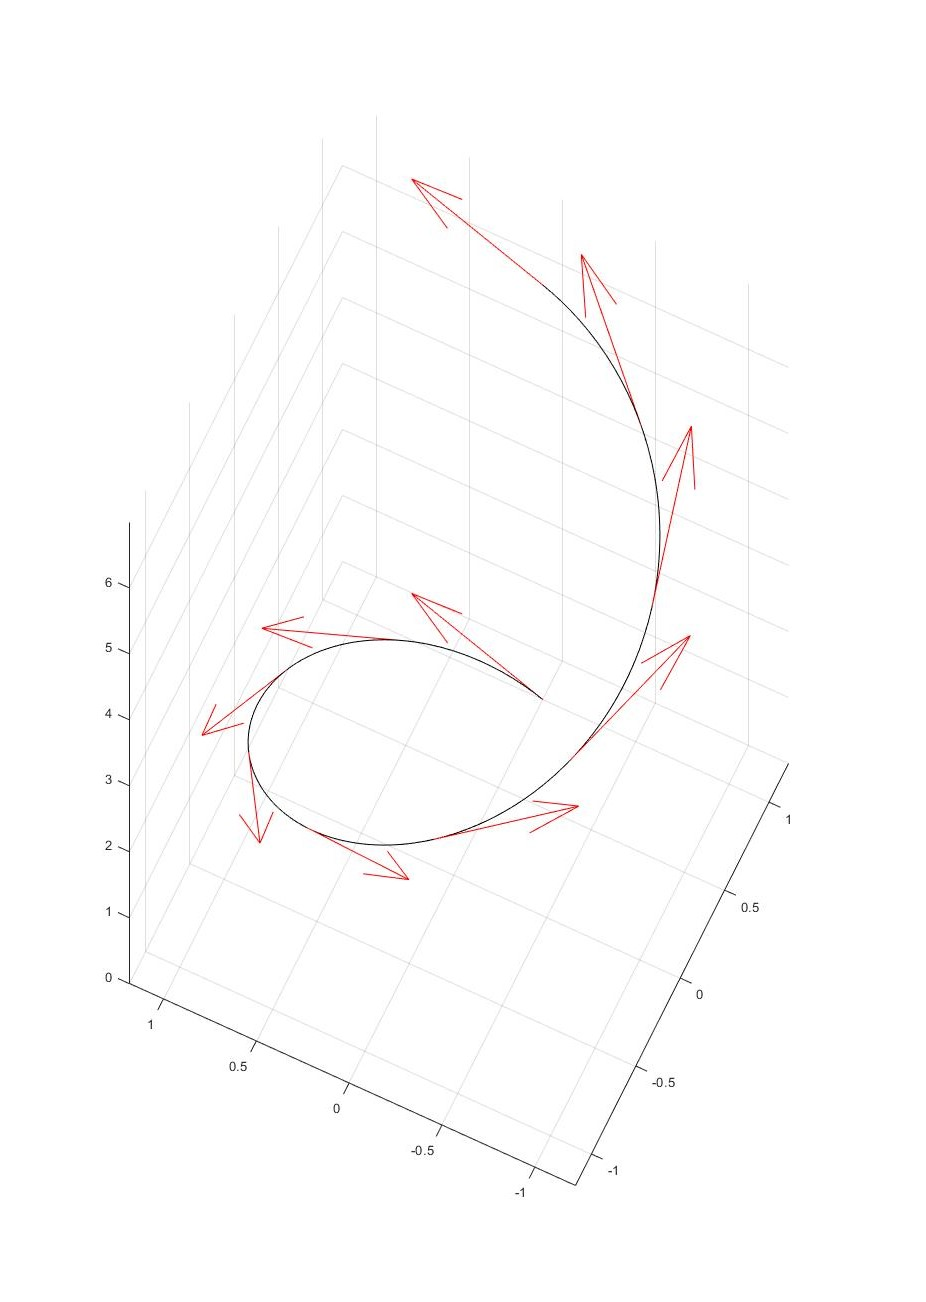
\includegraphics[scale=0.2]{C:/Users/Acer/Desktop/diploma/Diploma/slike/FrenetOgrodjeTangenta'.jpg} &
	\includegraphics[scale=0.2]{C:/Users/Acer/Desktop/diploma/Diploma/slike/FrenetOgrodje3'.jpg}
	\end{array}
	\end{equation*}
	Na sliki \ref{tan} je prikazan tangentni vektor, na sliki \ref{fogrodje} pa krivulja z Frenetovim ogrodjem.
\end{primer}
\begin{definicija}
Ogrodje $(\e_1,\e_2,\e_3)$ je usmerjeno, če $\e_1$ v vsaki točki krivulje kaže proti izhodišču koordinatnega sistema.
\end{definicija}
\begin{equation*}
\begin{array}{c c}
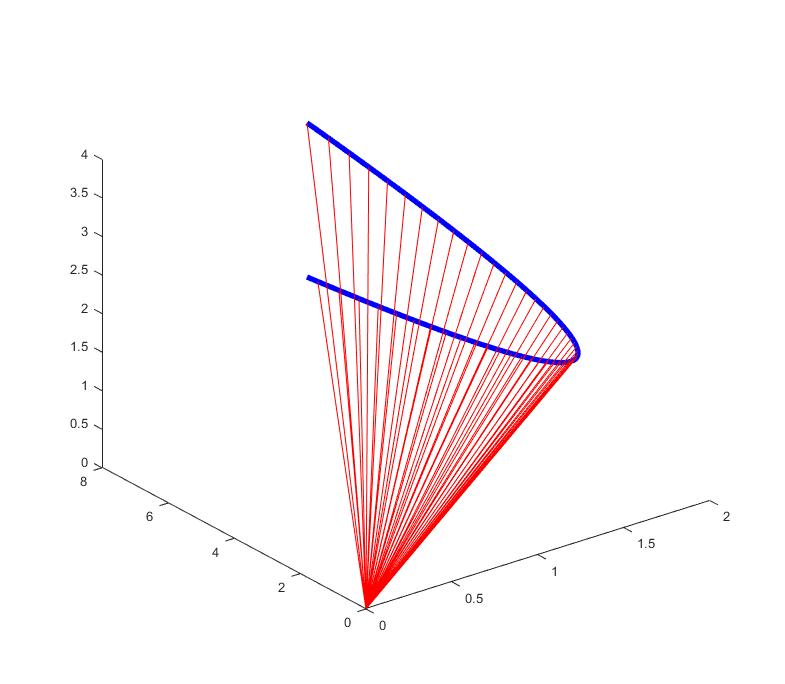
\includegraphics[scale=0.25]{C:/Users/Acer/Desktop/diploma/Diploma/slike/polarindi1.jpg} &
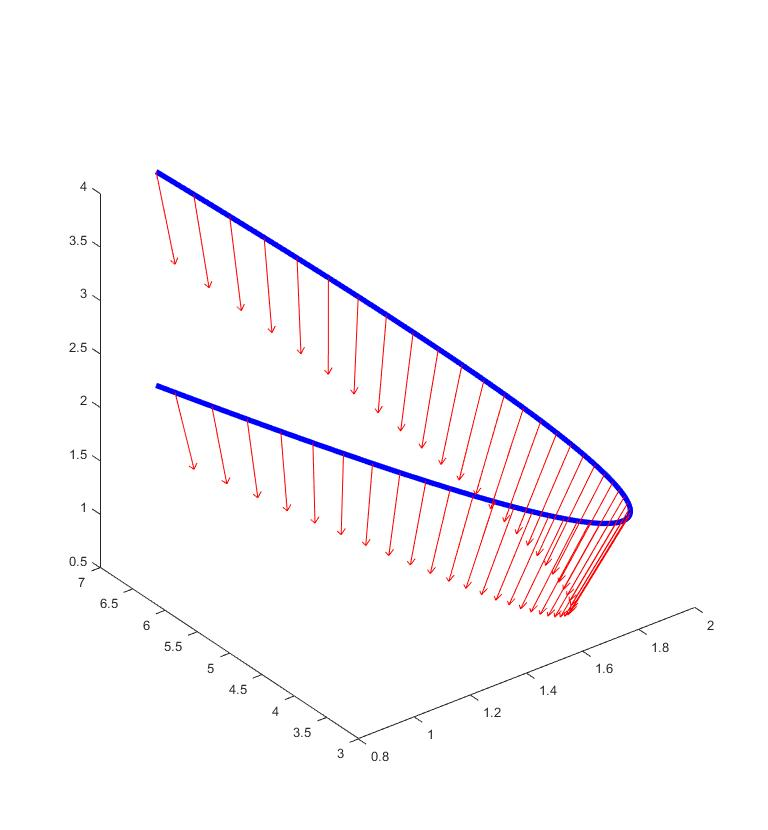
\includegraphics[scale=0.25]{C:/Users/Acer/Desktop/diploma/Diploma/slike/polarindi4.jpg}
\end{array}
\end{equation*}
Na zgornjih slikah vidimo krivuljo in vektor $\e_1$, ki vedno kaže proti izhodišču. 
\begin{opomba}
	Vektor $\e_1$ imenujemo polarni indikator.
\end{opomba}
Sedaj, ko smo si pogledali obe vrsti ogrodij, je seveda jasno, katero ogrodje si bomo izbrali pri naši konstrukciji. Ker si želimo opisati gibanje kamere, ki bo ves čas potovanja po krivulji snemala nek fiksen objekt v izhodišču, si izberemo usmerjeno ogrodje in položaj kamere orientiramo skladno z danim ogrodjem.

\subsection{Rotacijsko minimizirajoča ogrodja} Pojem se povezuje z dejstvom, da si želimo čim manj nepotrebnih rotacij samega ogrodja okoli izbrane osi. Bolj natančno, vektorja $\e_2$ in $\e_3$, ki razpenjata normalno ravnino, naj nimata nobene nenadne rotacije okoli vektorja $\e_1$. Poglejmo si primer na Frenetovem ogrodju.
\begin{primer}
	Če določimo krivuljo, je s tem določem tudi njen tangentni vektor. Kaj pa druga dva vektorja, ki določata ogrodje? Prikrojeno ogrodje je definirano tako, da vektorja v normalni ravnini nista fiksirana. Problem je v tem, da ju lahko zarotiramo za poljuben kot, tako dobljeni vektorji, pa še vedno tvorijo ogrodje. Torej vektorja $\e_2$ in $\e_3$ lahko izberemo kot poljubni rotaciji vektorjev $\NN$ in $\BB$, za poljuben kot $\phi$:
	\begin{equation*}
		\begin{bmatrix}
		\e_2 \\
		\e_3
		\end{bmatrix}
		=
		\begin{bmatrix}
		\cos \phi & \sin \phi \\
		-\sin \phi & \cos \phi
		\end{bmatrix}
		\begin{bmatrix}
		\NN \\ \BB
		\end{bmatrix}.
	\end{equation*}
\begin{equation*}
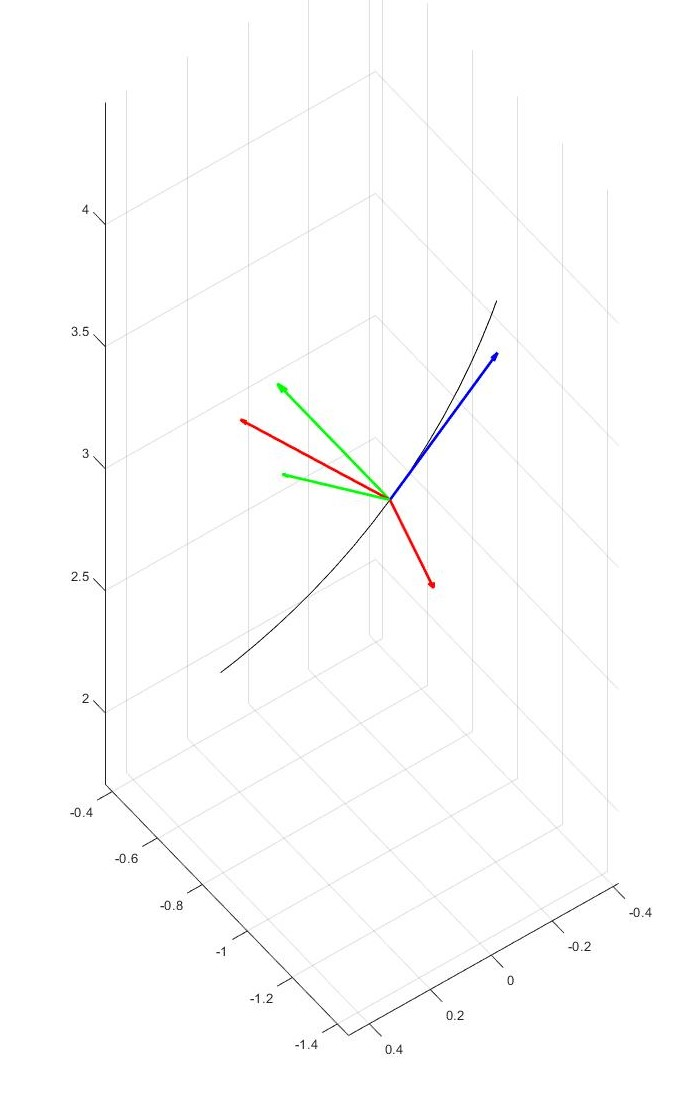
\includegraphics[scale=0.25]{C:/Users/Acer/Desktop/diploma/Diploma/slike/dvaOgrodja'.jpg}
\end{equation*}
Na sliki \ref{dvaogrodja} vidimo tak primer. Modri tangentni vektor $\TT$, in zelena $\NN$ in $\BB$ tvorijo prikrojeno ogrodje. Vendar prav tako tvorijo prikrojeno ogrodje moder vektor $\TT$ in rdeča $\NN$ in $\BB$.
\end{primer}
Torej, izmed vseh možnih ortonormiranih ogrodij, ki jih lahko konstruiramo na krivulji, nas bodo zanimala le taka, ki nam zagotovijo čim manj rotacij v ravnini, ki je pravokotna  na $\e_1$.
 
Vsako ogrodje ima neko kotno hitrost $\omega$, ki nam pove, kako se ogrodje spreminja, oziroma kako se spreminjata vektorja $\e_2$ in $\e_3$.
\begin{definicija}
Naj bo $(\e_1,\e_2,\e_3)$ ogrodje in $\omega$ pripadajoča kotna hitrost. Potem je $\omega$ definirana z naslednjimi diferencialnimi enačbami:
\begin{equation}
\frac{d\e_i}{dt}(t) = \omega(t) \times \e_i(t), ~~ i=1,2,3.
\end{equation}
\end{definicija}

Ker se bomo v nadaljevanju ukvarjali samo z usmerjenimi ogrodji, si poglejmo povezavo med le temi.
\begin{definicija}
Usmerjeno ogrodje $(\e_1,\e_2,\e_3)$ je rotacijsko minimizirajoče, če velja $\langle \omega,\e_1\rangle = 0.$
\end{definicija}

\begin{trditev}
Ogrodje $(\e_1,\e_2,\e_3)$, definirano kot 
\begin{equation}{\label{ERogrodje}}
\begin{array}{c c c}
\e_1 = \frac{\A\ii\overline{\A}}{\A\overline{\A}}, &
\e_2 = \frac{\A\jj\overline{\A}}{\A\overline{\A}}, &
\e_3 = \frac{\A\kk\overline{\A}}{\A\overline{\A}},
\end{array}
\end{equation}
je ortonormirana baza prostora $\R^3$.
\end{trditev}
\begin{opomba}
	Ogrodje \ref{ERogrodje} imenujemo Euler-Rodroguesovo ogrodje.
\end{opomba}
\begin{dokaz}
Pokazati moramo, da so skalarni produkti $\langle \e_i, \e_j \rangle $ enaki 0, za $i, j = 1,2,3, i \neq j$. Vemo, da so skalarni deli $\e_1,\e_2,\e_3$ enaki 0, zato lahko uporabimo formulo \ref{mn_kvat_0} za skalarni produkt dveh čistih kvaternionov. Dobimo
\begin{equation*}
\begin{split}
	\langle \e_1,\e_2 \rangle& = -scal \left( \e_1 \cdot \e_2 \right) \\
	& = -scal \left( \A \ii \overline{\A} \A \jj \overline{\A} \right) \\
	&= - ||\A||^2 scal \left( \A \ii \jj \overline{\A} \right) \\
	& = - ||\A||^2 scal \left( \A \kk \overline{\A} \right) \\
	& = 0.
\end{split}
\end{equation*}
Analogno pokažemo, da je $\langle \e_2,\e_3 \rangle = 0$, $\langle \e_1,\e_3 \rangle = 0$.
Izračunajmo še dolžie vektorjev $\e_1,\e_2,\e_3$. Za $\e_1$ velja
\begin{equation*}
\begin{split}
\A \ii \overline{\A} \A \ii \overline{\A} 	&= ||A||^2 \A \ii^2 \overline{\A} \\
	&= -||A||^4.
\end{split}
\end{equation*}
Od tod sledi
\begin{equation*}
\begin{split}
	\langle \e_1,\e_1 \rangle &= -scal \left( \e_1 \cdot \e_1 \right) \\
&= -scal (-\frac{1}{||\A||^4}||A||^4) \\
&= 1.
\end{split}
\end{equation*}
Na isti načim pokažemo, da velja $||\e_2||=||\e_3||=1$, od koder sledi, da je res ortonormirana baza v $\R^3$.
\end{dokaz}
\begin{trditev}{\label{rot_min}} Recimo, da imamo ogrodje definirano kot zgoraj.
	Usmerjeno ogrodje je rotacijsko minimizirajoče natanko tedaj, ko je $scal(\A' i\overline{\A})\equiv0$.
\end{trditev}
\begin{dokaz}
Želimo pokazati, da velja
\begin{equation}
\langle \omega,\e_1\rangle = 0 \Leftrightarrow scal(\A' \\i\overline{\A}) = 0.
\end{equation}
Razvijemo $\omega$ po bazi $\left(\e_1,\e_2,\e_3\right)$: $\omega = \omega_1\e_1+\omega_2\e_2+\omega_3\e_3$. Torej velja
\begin{equation*}
\langle \omega, \e_1 \rangle = \langle \omega_1\e_1,\e_1\rangle + \langle \omega_2\e_2,\e_1\rangle + \langle \omega_3\e_3,\e_1\rangle= \omega_1\langle \e_1,\e_1\rangle + \omega_2\langle \e_2,\e_1\rangle + \omega_3\langle \e_3,\e_1\rangle
\end{equation*}
Ker so $\e_1,\e_2,\e_3$ ortogonalni, je  $\langle \e_2,\e_1\rangle = 0$ in $\langle \e_3,\e_1\rangle=0$.
Ostane nam
\begin{equation*}
\langle \omega,\e_1 \rangle =\omega_1 || \e_1 ||^2 = \omega_1,
\end{equation*}
od koder vidimo, da je $\langle \omega, \e_1\rangle = 0$ natanko tedaj, ko je $\omega_1 = 0$.
Po definiciji velja
\begin{equation*}
\frac{d\e_i}{dt}(t) = \omega(t) \times \e_i(t), ~~ i=1,2,3.
\end{equation*}
Razpišimo enačbe posebej. Za $i=1$ dobimo
\begin{equation*}
\e_1' = \omega \times \e_1 = (\omega_1 \e_1 + \omega_2 \e_2 + \omega_3 \e_3) \times \e_1
= \omega_2 \e_2 \times \e_1 + \omega_3 \e_3 \times \e_1 = - \omega_2\e_3 + \omega_3\e_2.
\end{equation*}
Celotno enačbo skalarno pomnožimo najprej z $\e_2$, nato z $\e_3$ in upoštevamo da so $\e_1,\e_2,\e_3$ ortogonalni. Dobimo:
\begin{equation*}
\langle \e_1', \e_2 \rangle  = \omega_3, \quad
\langle \e_1', \e_3 \rangle = -\omega_2.
\end{equation*}
Za $i=2$ velja
\begin{equation*}
\e_2' = \omega \times \e_2 = (\omega_1 \e_1 + \omega_2 \e_2 + \omega_3 \e_3) \times \e_2 =
\omega_1 \e_1 \times \e_2 + \omega_3 \e_3 \times \e_2
=\omega_1\e_3 -\omega_3\e_1.
\end{equation*}
Podobno kot prej enačbo skalarno pomnožimo z $\e_1$ in $\e_3$. Dobimo
\begin{equation*}
\langle \e_2', \e_1 \rangle  = -\omega_3, \quad 
\langle \e_2', \e_3 \rangle = \omega_1.
\end{equation*}
Za $i=3$ velja
\begin{equation*}
\e_3' = \omega \times \e_3 = (\omega_1 \e_1 + \omega_2 \e_2 + \omega_3 \e_3) \times \e_3 =
\omega_1 \e_1 \times \e_3 + \omega_2 \e_2 \times \e_3
= - \omega_1\e_2 + \omega_2\e_1
\end{equation*}
Ponovno enačbo skalarno pomnožimo, tokrat z $\e_1$ in $\e_2$. Dobimo
\begin{equation*}
\langle \e_3', \e_1 \rangle  = \omega_2, \quad
\langle \e_3', \e_2 \rangle = -\omega_1
\end{equation*}
Dobljene rezultate združimo in dobimo zveze
\begin{equation}
\begin{split}
\omega_1 &= \langle \e_2', \e_3 \rangle = - \langle \e_3', \e_2 \rangle, \\
\omega_2 &= \langle \e_1', \e_3 \rangle = - \langle \e_3', \e_1 \rangle, \\
\omega_3 &= \langle \e_1', \e_2 \rangle = - \langle \e_2', \e_1 \rangle. 
\end{split}
\end{equation}
Na tej točki določimo naše ogrodje.
\begin{equation*}
\begin{array}{c c c}
\e_1 = \frac{\A \ii \overline{\A}}{\A \overline{\A}} &
\e_2 = \frac{\A \jj \overline{\A}}{\A \overline{\A}} &
\e_3 = \frac{\A \kk \overline{\A}}{\A \overline{\A}}
\end{array}
\end{equation*}
Vemo, da tvorijo ortonormirano bazo. Vemo tudi, da ima produkt $\A \ii \overline{\A}$ skalarni del enak 0. Enako poračunamo za $\A \jj \overline{\A}$ in $\A \kk \overline{\A}$. Od tu sledi:
\begin{equation*}
\begin{split}
	\omega_1 = \langle \e_2', \e_3 \rangle& = -skal \left( \left( \A \jj \overline{\A} \right)' \cdot \left( \A \kk \overline{\A}  \right) \right) \\
	&= -skal \left( \left( \A' \jj \overline{\A} + \A \jj \overline{\A}' \right)' \cdot \left( \A \kk \overline{\A}  \right) \right) \\
	&= -skal \left( \left( \A' \jj \overline{\A} \A \kk \overline{\A}+ \A \jj \overline{\A}' \A \kk \overline{\A}  \right) \right) \\
	&= -skal \left( ||\A||^2 \A' \ii \overline{\A}+ \overline{\left(\A' \overline{\jj} \overline{\A}\right)} \overline{ \left( \A \overline{\kk} \overline{\A} \right) }\right) \\
	&= -skal \left( ||\A||^2 \A' \ii \overline{\A}+ \overline{\left( ||\A||^2 \A' \overline{\ii} \overline{\A}\right)} \right) \\
	&= -skal \left( ||\A||^2 \A' \ii \overline{\A} \right)-skal \left(\left( ||\A||^2 \A \ii \overline{\A}'\right) \right) \\
	&= -2||\A||^2 skal \left( \A' \ii \overline{\A}\right).
\end{split}
\end{equation*}
Od tod sledi
\begin{equation*}
\omega_1 = 0 \Leftrightarrow skal \left( \A' \ii \overline{\A} \right) = 0,
\end{equation*}
kar zaključuje dokaz.
\end{dokaz}
\begin{opomba}{\label{aq}}
V splošnem to ogrodje ne bo rotacijsko minimizirajoče, če poljubeno izberemo kvaternionski polinom $\A$. Iz $\A$ lahko izpeljemo novo ogrodje, ki bo tudi usmerjen in bo rotacijsko minimizirajoče. Definiramo nov kvaternionski polinom $\B$ s predpisom: $\B(t) = \A(t) \QQ(t)$, kjer je $\QQ$ tak kvaternionski polinom, da velja $\QQ(t) \ii \overline{\QQ(t)} = \left( \QQ(t) \overline{\QQ(t)} \right) \ii$. Tako dobimo:
\begin{equation*}
	\B \ii \overline{\B} = \A \QQ \ii \overline{\QQ} \overline{\A} = \A \QQ \overline{\QQ} \ii \overline{\A} = ||\QQ||^2\A\ii\overline{\A}.
\end{equation*}
Torej bo smer vektorja $\frac{\B \ii \overline{\B}}{\B  \overline{\B}}$ enaka smeri vektorja $\frac{\A \ii \overline{\A}}{\A  \overline{\A}}$, kar pomeni, da bo ogrodje res usmerjeno ogrodje. Torej $\QQ$ doličimo tako, da bo $\B = \A\QQ$ določalo rotacijsko minimizirajoče ogrodje. S pomočjo kvaternionskega polinoma $\QQ$, lahko dobimo več prostih parametrov pri konstrukciji krivulje. Višja kot bo stopnja $\QQ$, več le teh dobimo. V nadaljevanju bomo zaradi lažje analize predpostavili, da je $\QQ=1$.
\end{opomba}

\iffalse

\begin{izrek}
Naj bo $e$ enotski vektor, $d$ neničelni vektor. Rešitev enačbe $\A e \overline{\A} = b$, kjer je $\A$ kvaternionski polinom, je:
\begin{equation*}
	\A = \sqrt{|b|} \frac{e+\frac{b}{|b|}}{|e+\frac{b}{|b|}|} \left( cos \phi + e sin\phi \right),
\end{equation*}
kjer je $\phi$ prost kotni parameter.
\end{izrek}

\begin{dokaz}
	TODO
\end{dokaz}

Konstruirali bomo P-krivuljo $\rr(t)$ stopnje 4, ki bo interpolirala naslednje podatke:\\
Začetni položaj:
\begin{equation}
	\rr(0) = \oo_z, ~~~~~ \rr(1) = \lambda \oo_k
\end{equation}
Začetno ogrodje:
\begin{equation}
\begin{split}
	(\oo(0),\uu(0), \vv(0)) = (\oo_z, \uu_z, \vv_z)\\
(\oo(1),\uu(1), \vv(1)) = (\oo_k, \uu_k, \vv_k)
\end{split}
\end{equation}
Začetna tangenta, smer
\begin{equation}
	\rr '(0) = \mu \ff_z
\end{equation}
Prav tako, mora za krivuljo $\rr(t)$ obstajati rotacijsko minimizirajoče ogrodje.\\
Brez škode za splošnost, postavimo za začetno ogrodje $(\oo_z, \uu_z, \vv_z) = (\ii, - \jj, -\kk)$ in nastavimo $\g_z = \ii \times \ff_z$. Vemo, da bo naša krivulja oblike $\rr(t) = \A(t) \ii \overline{\A(t)}$. Izrazimo začetne podatke z komponentami kvaternionskega polinoma $\A(t) = \A_0(1-t)^2 + \A_02(1-t)t + \A_2t^2$.Iz primera (?) vemo, da se začetna in končna točka izražata kot:
\begin{equation}
	\begin{split}
	\rr(0) = \A_0 \ii\overline{\A_0} = \oo_z = \ii \\
		\rr(1) = \A_2 \ii\overline{\A_2} = \lambda \oo_k \\
	\end{split}
\end{equation}
Poračunajmo še tretji pogoj:
\begin{equation*}
\begin{split}
	\rr'(t) &= \A(t)' \ii \overline{\A(t)} + \A(t) \ii \overline{\A(t)}' \\
	\A(t)' &= \A_02(1-t)(-1) + \A_12(1-t) - \A_12t + \A_2 2t \\
	\A(0)' &= -\A_0 + 2 \A_1 \\
	\rightarrow \rr(0)' &= 2(\A_1-\A_0)\ii \overline{\A_0} + \A_0 \ii 2(\overline{\A_1} - \overline{\A_0}) \\
	&= 2\A_1 \ii \overline{\A_0} - 2 \A_0 \ii \overline{\A_0} + 2 \A_0 \ii \overline{\A_1}-2\A_0 \ii \overline{\A_0} \\
	&= 2(\A_0 \ii \overline{\A_1} + \A_1 \ii \overline{\A_0}) - 4 \A_0 \ii \overline{\A_0} \\
	&= 2(\A_0 \ii \overline{\A_1} + \A_1 \ii \overline{\A_0}) - 4 \ii \\
	&= \mu \ff_z
\end{split}
\end{equation*}
Torej:
\begin{equation}
	\mu \ff_z + 4 \ii = 2(\A_0 \ii \overline{\A_1} + \A_1 \ii \overline{\A_0})
\end{equation}
Po izreku (?) je rešitev zgornjih dveh enačb (?) enaka:
\begin{equation}
	\A_0 = \ii (cos\phi_0 + \ii sin \phi_0),
\end{equation}
ker imamo vzporedne vektorje, in
\begin{equation}
\begin{array}{c c}
	\A_2 = \sqrt{|\lambda|} \frac{\ii + \lambda}{|\ii + \lambda|}(cos\phi_2 + \ii sin\phi_2),
\end{array}
\end{equation}
če je $\oo_k != -1$, in 
\begin{equation}
\A_2 = \sqrt{|\lambda|} \jj(cos\phi_2 + \ii sin\phi_2)
\end{equation}
sicer. Brez škode za splošnost nastavimo $\phi_0 = 0$. Iz tega sledi, da je $\A_0 = \ii$.
\begin{izrek}
	Za P-krivuljo, ki jo določa kvaternionski polinom $\A(t) = \A_0(1-t)^2 + \A_02(1-t)t + \A_2t^2$, obstaja rotacijsko minimizirajoče ogrodje, če velja:
	\begin{equation}
		\A_1 \ii \overline{\A_1} = vect(\A_2 \ii \overline{\A_0}).
	\end{equation}
\end{izrek}
\begin{dokaz}
	TODO
\end{dokaz}
Zaradi bolše preglednosti, vpeljimo nove oznake.
\begin{equation}
\begin{array}{c c}
	\A_2 = \sqrt{|\lambda|} n_2 (cos\phi_2 + \ii sin\phi_2) &, n_2 = \frac{\ii + \lambda}{|\ii + \lambda|}
\end{array}
\end{equation}
Torej se pogoj (?) pretvori v
\begin{equation}
\begin{split}
	\A_1 \ii \overline{\A_1} &=vect(\A_2 \ii \overline{\A_0})\\  
	&=vect(\A_2) \\
	&= vect\left( \sqrt{|\lambda|} n_2(cos\phi_2 + \ii sin\phi_2) \right) \\
	&= \sqrt{\lambda} \left(n_2 cos\phi_2 + n_2 \times \ii sin\phi_2\right) 
\end{split}
\end{equation}
Ponovno uporabimo izrek (?) in dobimo rešitev za $\A_1$:
\begin{equation}
	\begin{array}{c c c}
	\A_1 = \sqrt{|w|} n_1(cos\phi_1 + \ii sin\phi_1), & w = \sqrt{\lambda} \left(n_2 cos\phi_2 + n_2 \times \ii sin\phi_2\right), & n_1 = \frac{w + |w| \ii}{|w + |w|\ii|}
	\end{array}
\end{equation}
Torej:
\begin{equation}
\begin{split}
	vect(\A_1) &= vec\left( \sqrt{|w|} n_1(cos\phi_1 + \ii sin\phi_1) \right) \\
	&=cos\phi_1 w_1 + sin\phi_1 w_2,
\end{split}
\end{equation}
kjer je
\begin{equation}
	\begin{array}{c c}
	w_1 = \sqrt{|w|} n_1, & w_2 = \sqrt{|w|} n_1 \times \ii
	\end{array}
\end{equation}
\begin{trditev}
	Če je $\oo_z != \ii$, so vektorji $w,~ w\times \ii,~ w_1,~w_2,~\g_z\times(w_1\times w_2)$ neničelni.
\end{trditev}
\begin{opomba}
	Trditev nam pove, da če je $\oo_z != \ii$, sta vektorja $w!=0$ in $w\times \ii != 0$ iz česar sledi, da sta $n_1$ in $\A_1$ dobro definirana.
\end{opomba}
\begin{dokaz}
	TODO
\end{dokaz}
Poračunajmo še eno enačbo. Iz (?) sledi:
\begin{equation}
	\begin{split}
	\mu \ff_z + 4 \ii &= 2(\A_0 \ii \overline{\A_1} + \A_1 \ii \overline{\A_0})\\
	&= 2(-\overline{\A_1} + A_1) \\
	&= 4vect(\A_1) \\
	\Longrightarrow vect(\A_1) &= \frac{\mu \ff_z}{4} + \ii
	\end{split}
\end{equation}
Ker je $\g_z = \ii \times \ff_z$ sledi:
\begin{equation}
	\langle vect(\A_1), \g_z\rangle = \langle \frac{\mu \ff_z}{4} + \ii ,\ii \times \ff_z \rangle = 
	\langle \frac{\mu \ff_z}{4} ,\ii \times \ff_z \rangle + 
	\langle \ii ,\ii \times \ff_z \rangle = 0
\end{equation}
\begin{equation}
	\langle vect(\A_1), \ff_z \rangle = \langle \frac{\mu \ff_z}{4} + \ii ,\ff_z \rangle = \frac{\mu}{4} > 0
\end{equation}

\fi



%%%%%%%%%%%%%%%%%%%%%%%%%%%%%%%%%%%%%%%%%%%%%%%%%%%%%%%%%%%%%%%%


\iffalse 

Ko sestavimo vse stvari skupaj, opišemo naš postopek z naslednjim algoritmom.\\
\textbf{Vhodni podatki:} začetna točka $\pp_z = d_z \oo_z$, končna točka $\pp_k = d_k \oo_k$, usmerjenost končnih točk $\left( \oo_z, \uu_z, \vv_z\right)$,  $\left( \oo_k, \uu_k, \vv_k\right)$, $\oo_z != \oo_k$.
\begin{enumerate}
	\item a
	\item b
\end{enumerate}
\fi

\section{Interpolacijski problem}{\label{int_problem}}
V tem razdelku bomo opisali interpolacijski problem, ki ga želimo interpolirati.
Opisali bomo konkreten postopek, kako dobiti P-krivuljo iz začetnih podatkov. 
 Poiskati želimo P-krivuljo, $\pp:\left[0,1\right] \rightarrow \R^3$, po predpisu $\pp(t) = \A(t)\ii\overline{\A(t)}$, kjer je $\A$ nek kvaternionski polinom. Za krivuljo $\pp$ naj velja, da je začetna točka enaka $\pp(0) = P_0$ in končna $\pp(1)=P_1$ in bo njeno rotacijsko minimizirajoče usmerjeno ogrodje pri $t=0$ enako $\left( \e_1^{z},\e_2^{z},\e_3^{z} \right)$, pri $t=1$ pa $\left( \e_1^{k},\e_2^{k},\e_3^{k} \right)$, pri čemer velja $\e_1^{z}= \frac{\pp(0)}{||\pp(0)||}$ in $\e_1^{k}= \frac{\pp(1)}{||\pp(1)||}$. Izkaže se, da če vzamemo linearni kvaternionski polinom $\A(t)$, potem ne moremo konstruirati rotacijsko minimizirajočega usmerjenega ogrodja \ref{neobstaja}. Zato bomo vzeli kvadraten kvaternionski polinom $\A(t)$.

	Najprej moramo rešiti enačbi, ki nam ju določata robna položaja.
	Prvi robni pogoj $\pp(0) = P_0$ nam da enačbo $\A_1 \ii \overline{\A_1} = P_0$, katere rešitev je po \ref{kvat_resitev} enaka 
	\begin{equation}
		\A_1(\phi_0) = \sqrt{||P_0||} \frac{\frac{P_0}{||P_0||}+\ii}{||\frac{P_0}{||P_0||}+\ii||} \left( \cos \phi_0 + \ii \sin \phi_0 \right),
	\end{equation}
	kjer je $\phi_0$ poljuben kot.
	Drugi robni pogoj $\pp(1) = P_1$ nam da enačbo $\A_2 \ii \overline{\A_2} = P_1$, katere rešitev je po \ref{kvat_resitev} enaka 
	\begin{equation}
	\A_2(\phi_2) = \sqrt{||P_1||} \frac{\frac{P_1}{||P_1||}+\ii}{||\frac{P_1}{||P_1||}+\ii||} \left( \cos \phi_2 + \ii \sin \phi_2 \right),
	\end{equation}
	kjer je $\phi_2$ poljuben kot.
	

	Zadostiti moramo pogoju za rotacijsko minimizirajoče ogrodje \ref{rot_min}.
	\begin{trditev} Naj bo $\A(t) = \A_0(1-t)^2 + \A_12(1-t)t+\A_2t^2$.
		Za krivuljo, definirano kot
		\begin{equation*}
			\pp(t) = \A(t)\ii\overline{\A(t)}
		\end{equation*}
		obstaja rotacijsko minimizirajoče usmerjeno ogrodje natanko tedaj, ko bo
		\begin{equation}{\label{rot_pogoj}}
			\A_1 \ii \overline{\A_1} = {\rm vect} \left(\A_2 \ii \overline{\A_0}\right).
		\end{equation}
	\end{trditev}
\begin{dokaz}
	Dokaz trditve je zelo zahteven in obsežen, zato ga izpustimo. Najdemo ga lahko v \ref{label}. Oglejmo si le, kako pridemo do iskanega rotacijsko minimizirajočega ogrodja. Kot smo že omenili v opombi \ref{aq}, za dan kvaternionski polinom $\A$, obstaja ER ogrodje, definiramo kot
	\begin{equation*}
		\e_1 = \frac{\B \ii \overline{\B}}{||\B||}, \quad \e_2 = \frac{\B \jj \overline{\B}}{||\B||}, \quad		\e_3 = \frac{\B \kk \overline{\B}}{||\B||},
	\end{equation*}
	kjer je $\B = \A \QQ$ in za $\QQ$ velja $\QQ\ii\overline{\QQ}= ||\QQ||\ii$.
	V \ref{} izvemo, da je $\QQ$ definiran kot $\QQ(t)= q_0-\ii q_1$, kjer sta $q_0$ in $q_1$ definirana kot
	\begin{equation}
		\begin{split}
		q_0(t) &= ||\A_0||^2(1-t)^2+{\rm scal} (\overline{\A_0}\A_1) 2t(1-t)+||\A_1||^2t^2, \\
		q_1(t) &=\langle \overline{\A_0} (\A_12t(1-t)+\A_2t^2)),(0,1,0,0) \rangle.
		\end{split}
	\end{equation}
\end{dokaz}
Iz enačbe \ref{rot_pogoj} poračunamo še koeficient $\A_1$. Po \ref{kvat_resitev} je ta enaka
\begin{equation}
	\A_1(\phi_2) = \sqrt{||b||} \frac{\frac{b}{||b||}+ \ii}{||\frac{b}{||b||}+ \ii||} \left(\cos \phi_1 + \sin \phi_1\right),
\end{equation}
kjer je $\phi_1$ poljuben kot in $b = {\rm vect} \left(\A_2 \ii \overline{\A_0}\right)$.



%%%%%%%%%%%%%%%%%%%%%%%%%%%%%%%%%%%%%%%%%%%%%%%%%%%%%%%%%%%%%%%%%%%%%%%%%%%%%%%%%%%%%%%%%%%%%%%%%%%%%%%%%5
\section{Numerični rezultati}
V tem poglavju si bomo ogledali nekaj numeričnih rezultatov, ki jih bomo dobili tako, da predpišemo začetni in končni položaj kamere in sledimo postopku opisanem v poglavju \ref{int_problem}. Če interpoliramo podatke, opisane v poglavju \ref{label}, potem dobimo tri proste parametre $\phi_0,\phi_1,\phi_2$, ki nam bodo določali končno krivuljo. 

\subsection{Primer 1}
\subsection{Primer 2}


\section*{Slovar strokovnih izrazov}

\geslo{adapted frame}{prikrojeno ogrodje}
\geslo{directed frame}{usmerjeno ogrodje}
\geslo{polar indicatries}{polarni indikator}
\geslo{rotation minimizing frame}{rotacijsko minimizirajoče ogrodje}

% seznam uporabljene literature
\begin{thebibliography}{99}
\bibitem{}R.T. Farouki, C. Giannelli, A. Sestini: \emph{An interpolation sceme for designing rational rotation-minimizing camera motions}(2011)
\bibitem{} R.T.Farouki, C.Gianelli: \emph{Spatial camera orientation control by rotation-minimizing directed frames}(2009)
\bibitem{} M. Krajnc, M.L. Samboli, A. Sestini, E. Žagar: \emph{$C^1$ interpolation by rational biarcs with rational rotation minimizing directed frames} (2014)
\bibitem{}{\label{neobstaja}} Han, C.Y.: \emph{Nonexistence of rational rotation-minimizing frames on cubic curves}. Comput. AidedGeom. Design25(4–5), 298–304 (2008)

\end{thebibliography}

\end{document}

